\subsection{Descrição dos sinais das entradas e saídas}

A figura~\ref{fig:visaogeral} é uma visão geral da comunicação entre o Kinect e
o FPGA.

\begin{figure}[h]
\centering
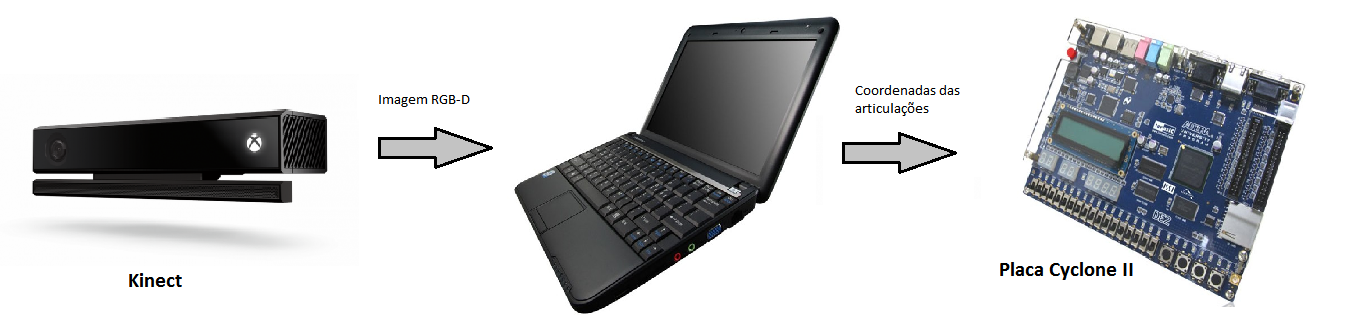
\includegraphics[width=.5\textwidth]{img/visao_geral}
\caption{Visão geral}
\label{fig:visaogeral}
\end{figure}


\begin{itemize}

\item \verb|clock|: é um pino de entrada para prover o sincronismo entre as
operações aritimeticas.

\item \verb|reset|: é um pino de entrada que reinicia o processo de calculo do
KNN. quando esta em 0 os registradores são reiniciados e a maquina de estados
vai para o estado inicial.

\item \verb|uart_rxd|: pino de recepção de dados da UART;

\item \verb|uart_txd|: pino de transmissão de dados da UART;

\item \verb|end_knn_out|: é um pino de saída que sinaliza quando 
terminou o calculo do KNN.

\end{itemize}